
\documentclass[border=3mm]{standalone}

\usepackage{tikz}
\usetikzlibrary{arrows,shapes.gates.logic.US,shapes.gates.logic.IEC,calc}
\begin{document}
\thispagestyle{empty}
\tikzstyle{branch}=[fill,shape=circle,minimum size=3pt,inner sep=0pt]
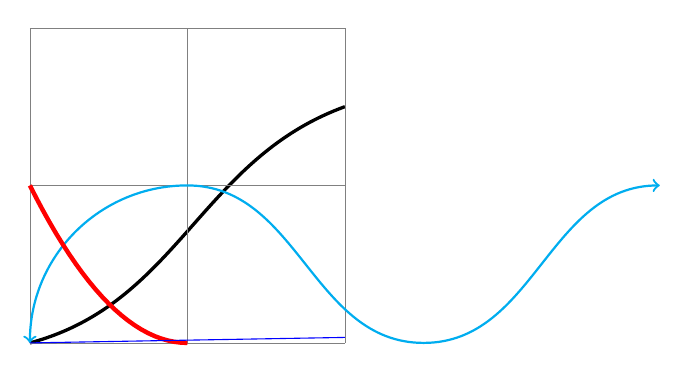
\begin{tikzpicture}[scale=2]

    \draw[very thick] (0,0) to [out=15,in=200] (2,1.5);
    \draw[help lines] (0,0) grid (2,2);

    \draw [<->,thick, cyan] (0,0) to [out=90,in=180] (1,1)
    to [out=0,in=180] (2.5,0) to [out=0,in=-180] (4,1) ;
    \draw[red, ultra thick, domain=0:1] plot (\x, {(\x-1)^2});
    \draw[blue, domain=0:2] plot (\x, {sin(\x)});
    

\end{tikzpicture}
\end{document} 